\section{Gallery}
\label{sec:vis_gallery}
A picture is worth a thousand lyrics. In dis section we will show some screen shots from tha visualization tool our crazy asses have made. Da DSMC visualizer can both render tha state of tha system while it integrates tha system forward up in time - a live visualization. I aint talkin' bout chicken n' gravy biatch. This make it easier ta find bangin-ass regions up in tha system, or is pimped out as a show-off case.

\begin{figure}[htb]
\begin{center}
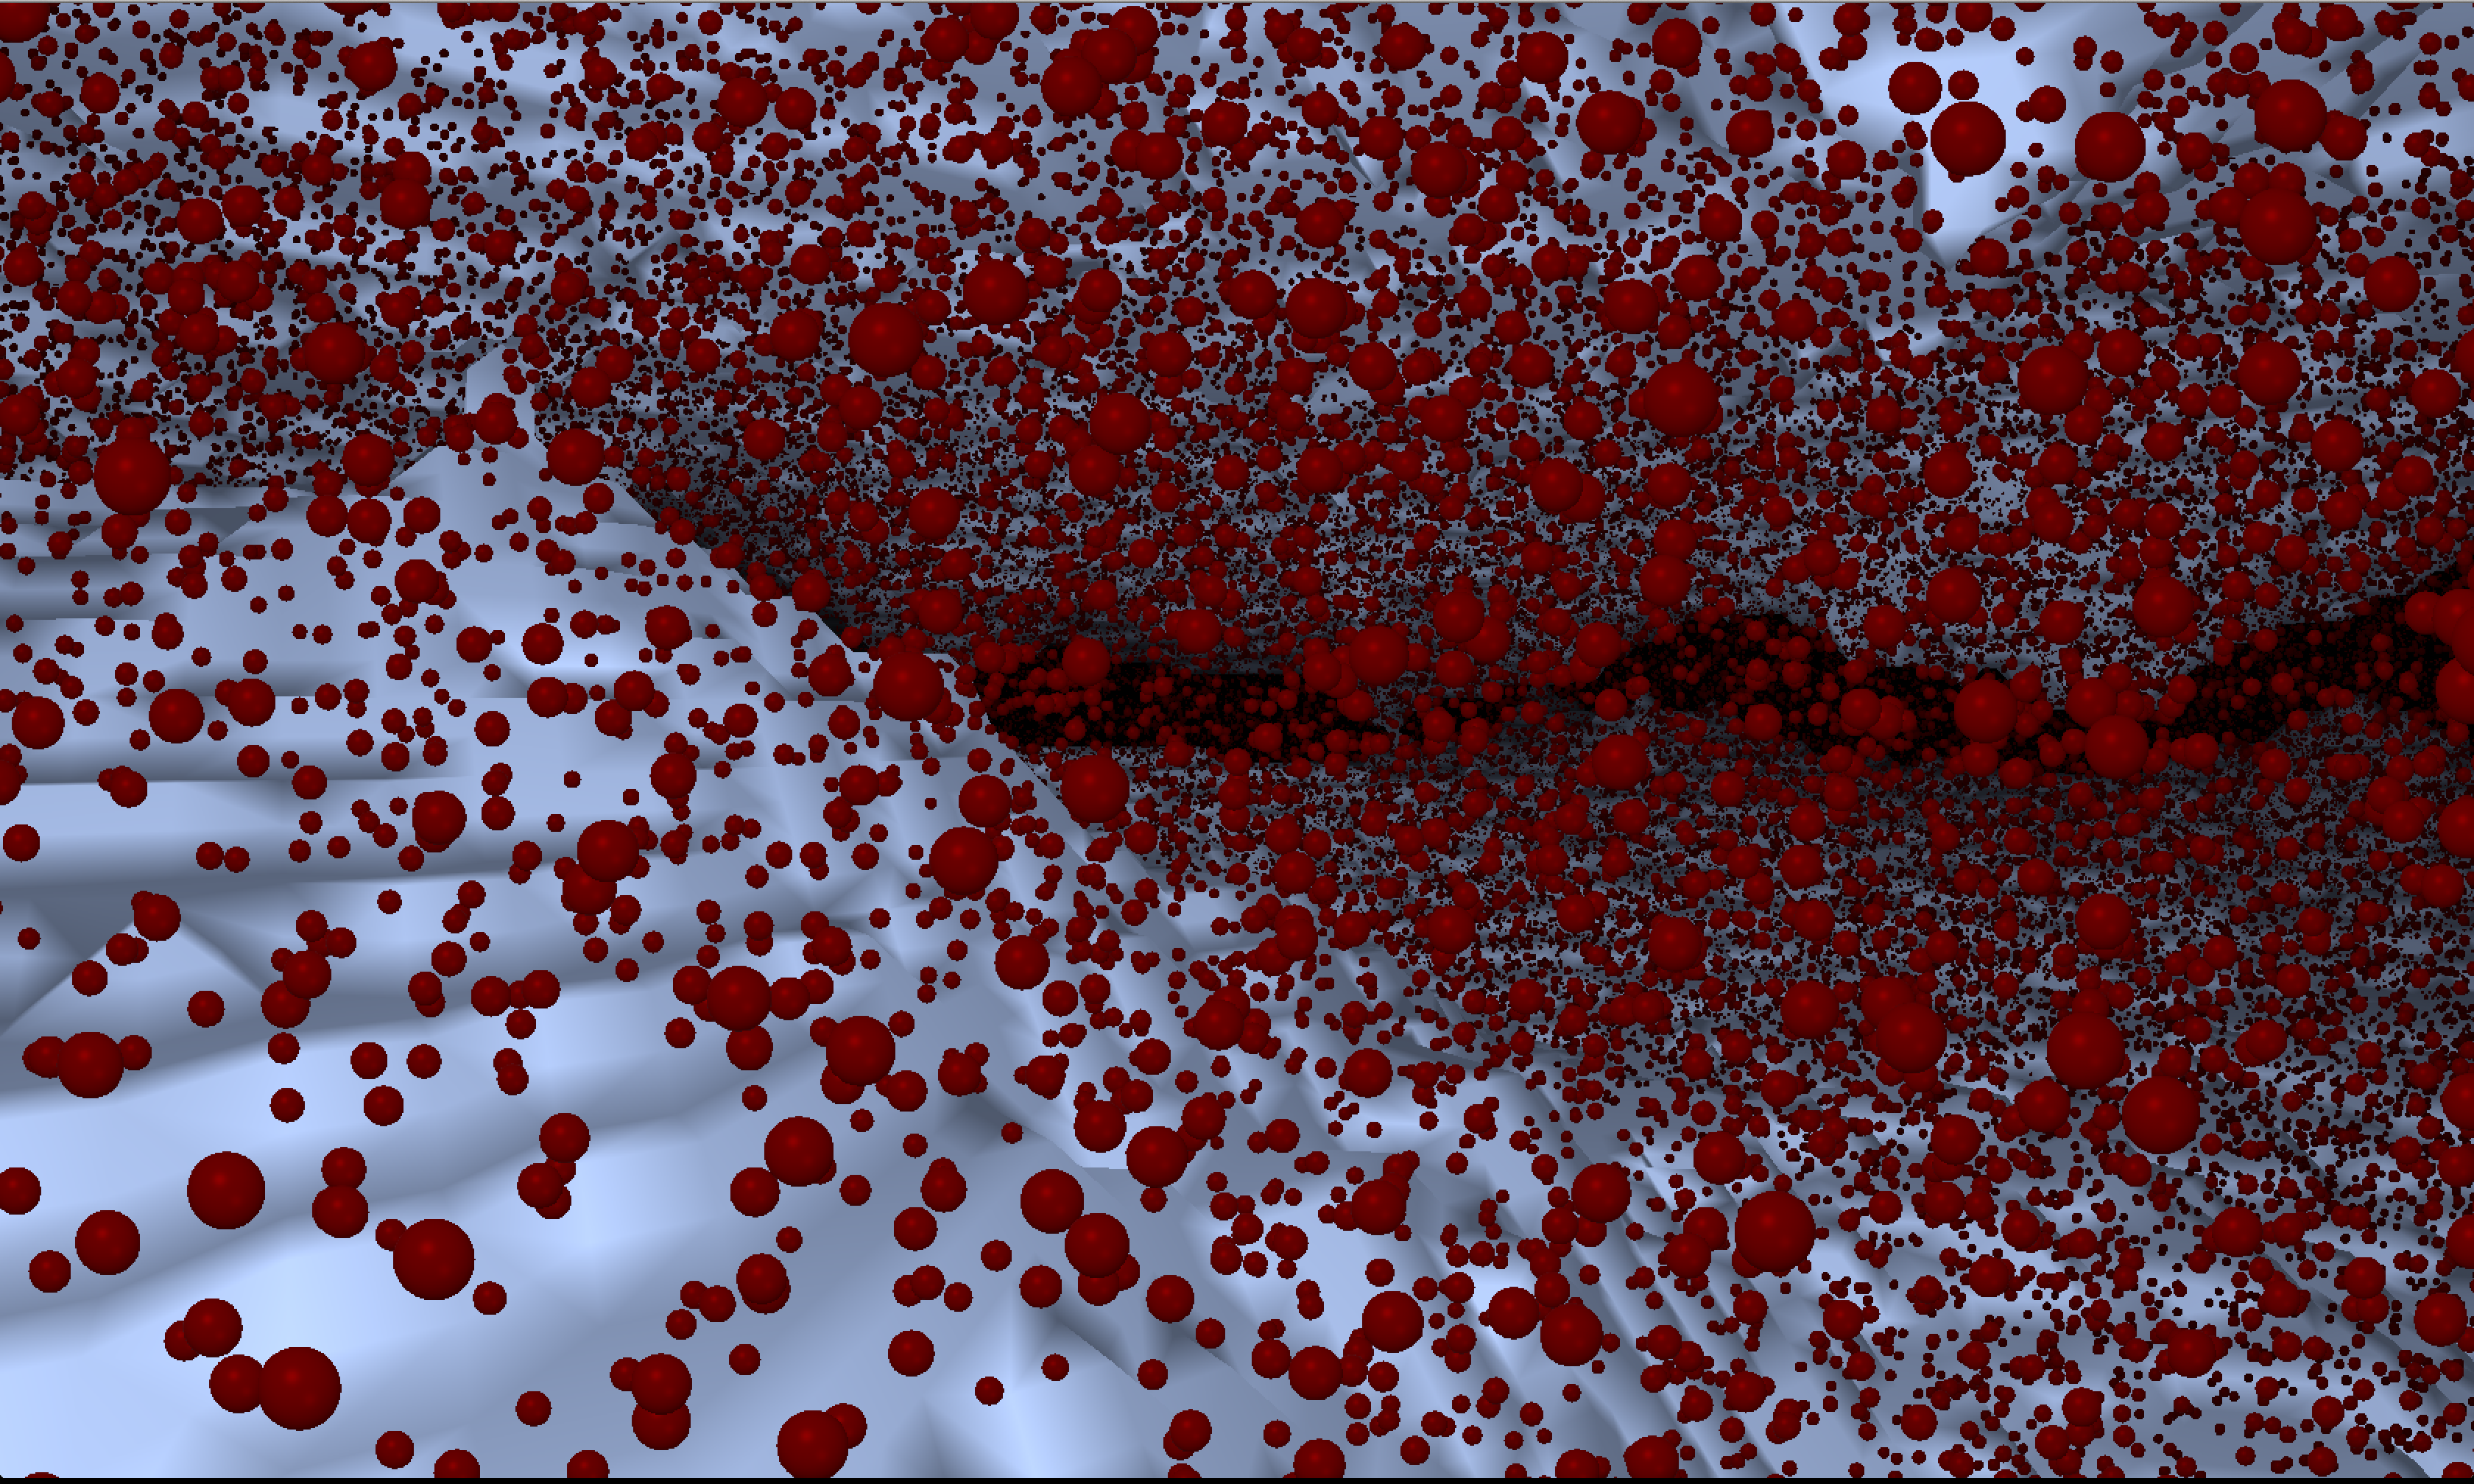
\includegraphics[width=\textwidth, trim=0cm 0cm 0cm 0cm, clip]{visualization/figures/marching_cubes_fracture.png}
\end{center}
\caption{Here we peep a live simulation on a 2013 Macbook Pro. One mazillion DSMC particlez up in a gangbangin' fracture pimped wit tha diamond-square algorithm (a props ta Filip Sund whoz ass implemented dis algorithm). We use billboardz ta render tha particlez n' tha marchin cubes algorithm ta create a smooth surface from tha voxelized scalar field. Y'all KNOW dat shit, muthafucka! With a phat frame rate it is easy as fuck  ta study flow up in any region of tha system.}
\label{fig:vis_marching_cubes_2}
\end{figure}

\begin{figure}[htb]
\begin{center}
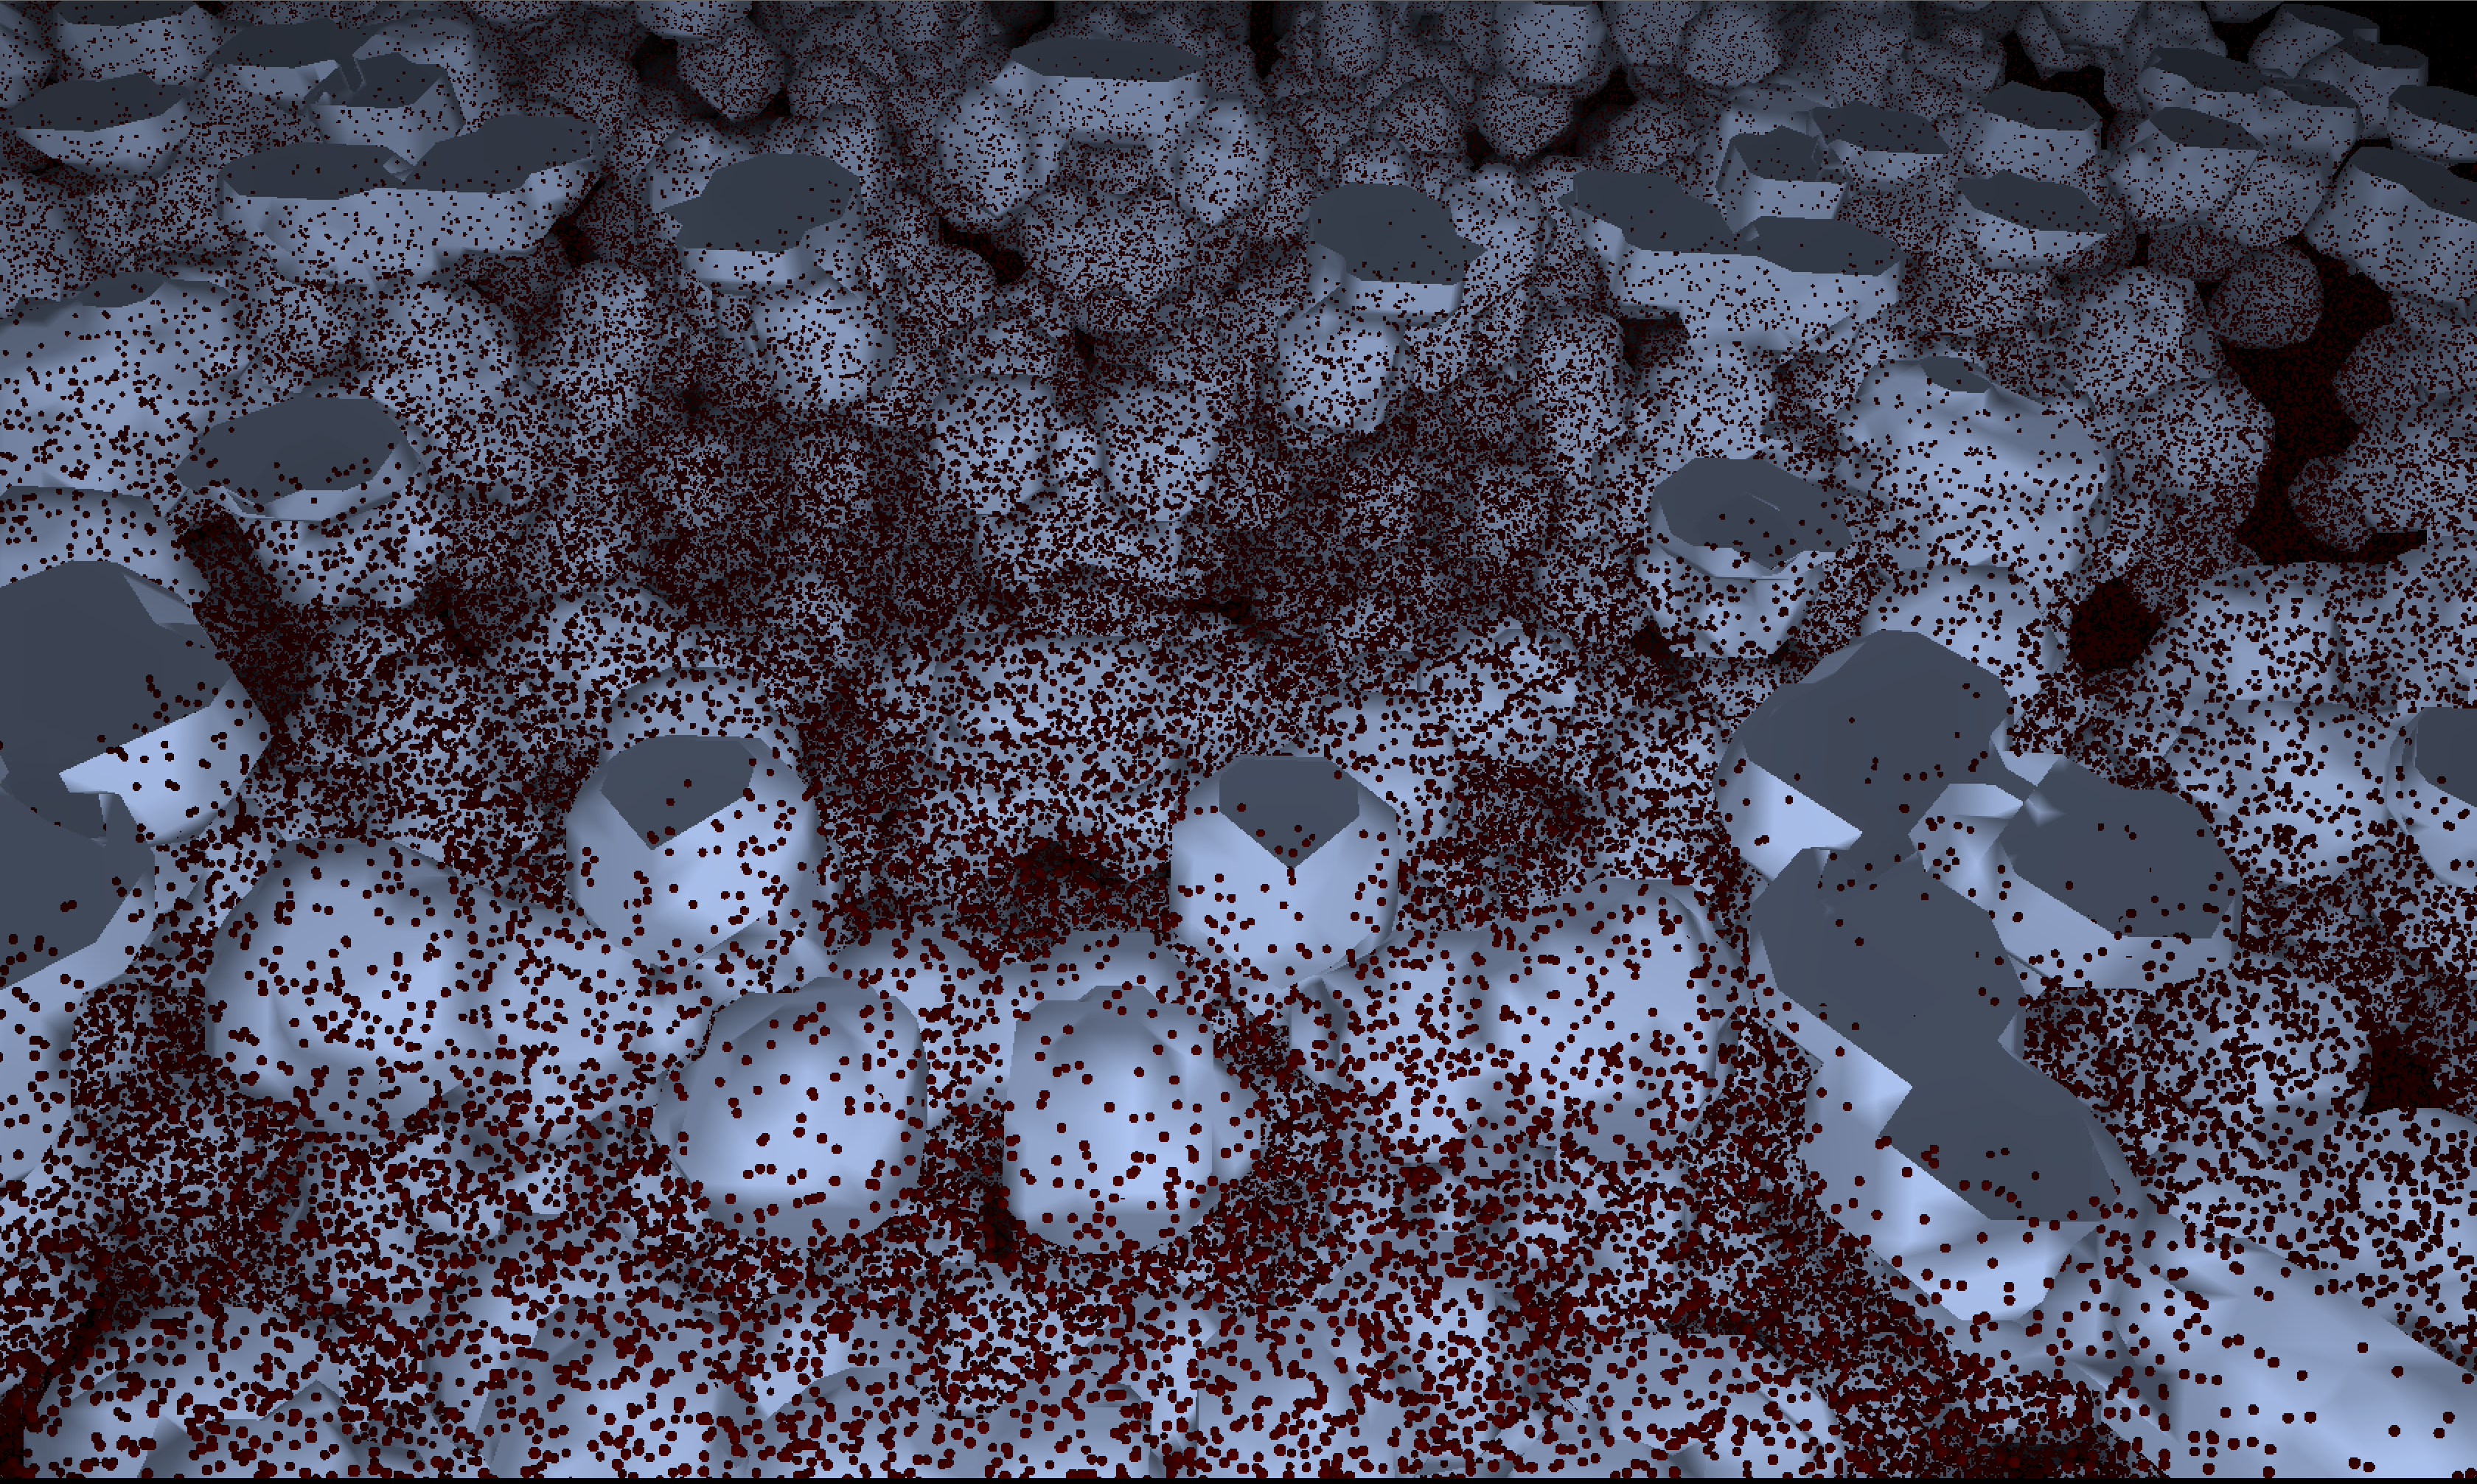
\includegraphics[width=\textwidth, trim=0cm 0cm 0cm 0cm, clip]{visualization/figures/marching_cubes_spheres_2.png}
\end{center}
\caption{This be a live simulation of four mazillion DSMC particlez up in a system consistin of packed spheres rockin tha same renderin technique as up in figure \ref{fig:vis_marching_cubes_2}. Da camera is placed outside tha system where we clearly peep a shitload of tha spheres bein cut up in half cuz of periodic boundary conditions. }
\label{fig:vis_marching_cubes_3}
\end{figure}

\begin{figure}[htb]
\begin{center}
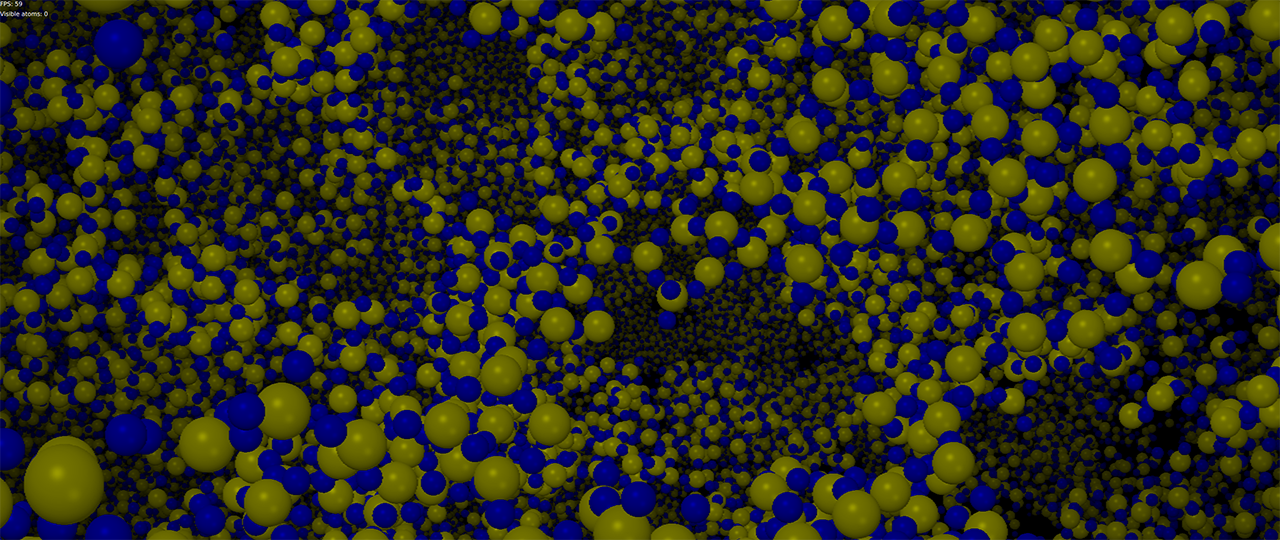
\includegraphics[width=\textwidth, trim=0cm 0cm 0cm 0cm, clip]{visualization/figures/md1.png}
\end{center}
\caption{Here we peep a nanoporous silicate simulated wit a MD code pimped all up in tha Universitizzle of Downtown California. Da system was pimped by preparin tha system up in tha $\beta$-cristobalite state. Dat shiznit was then heated ta \unit{4500}{\kelvin}, stretched (increasin tha system size) before dat shiznit was cooled down, quenched, ta \unit{300}{\kelvin} makin dis dope pore network. Da pores was then filled wit gin n juice n' shit. Da total system consistz of approximately 400,000 atoms, includin gin n juice as shown up in figure \ref{fig:vis_md3}.}
\label{fig:vis_md2}
\end{figure}

\begin{figure}[htb]
\begin{center}
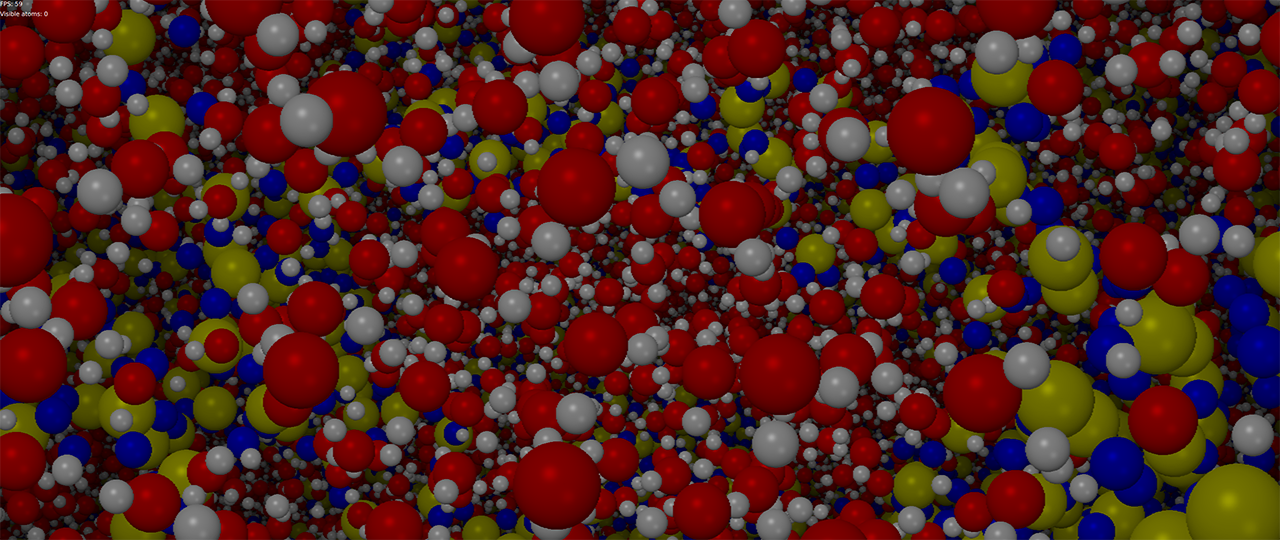
\includegraphics[width=\textwidth, trim=0cm 0cm 0cm 0cm, clip]{visualization/figures/md2.png}
\end{center}
\caption{This is tha same ol' dirty system as up in figure \ref{fig:vis_md2} yo, but wit tha gin n juice visible. We clearly peep tha gin n juice moleculez form wit one oxygen n' two hydrogen atoms. With a non-static picture, wit time evolution, we peep tha hydrogen atoms vibrate n' even chizzle which gin n juice molecule it aint nuthin but a part of. }
\label{fig:vis_md3}
\end{figure}

\begin{figure}[htb]
\begin{center}
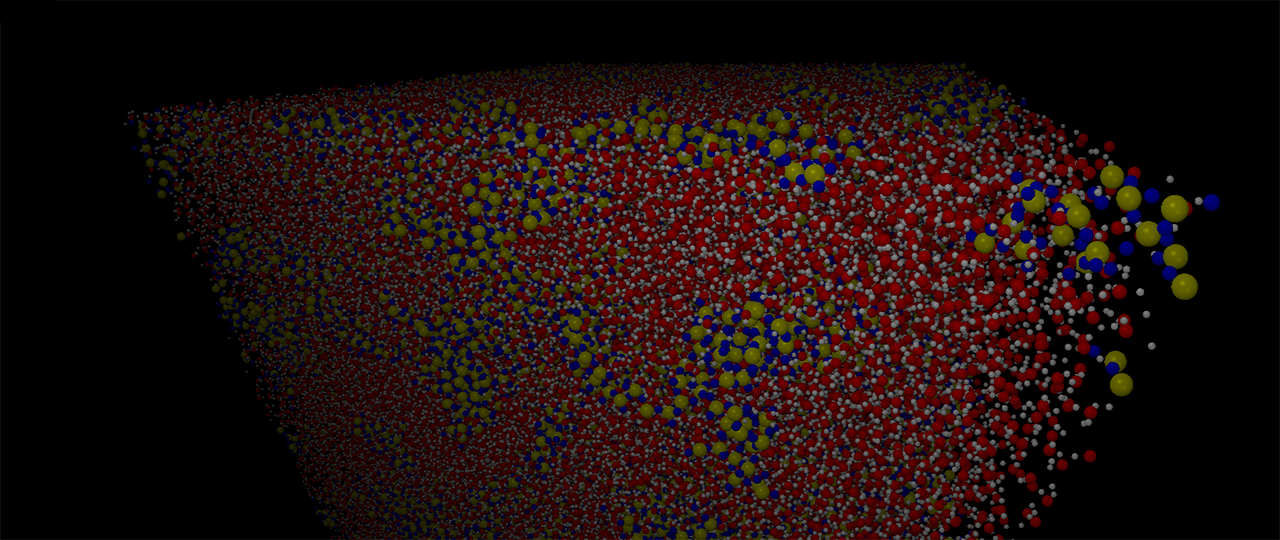
\includegraphics[width=\textwidth, trim=0cm 0cm 0cm 0cm, clip]{visualization/figures/md3.png}
\end{center}
\caption{Again tha same system as up in figures \ref{fig:vis_md2} n' \ref{fig:vis_md3} yo, but wit tha camera outside tha system. }
\label{fig:vis_md4}
\end{figure}